
\chapter{Réalisation du projet}

\section*{Introduction}
\addcontentsline{toc}{section}{Inroduction}

Ce chapitre est consacré à la présentation de la phase de réalisation du projet, en mettant en lumière les différentes étapes de développement et les choix techniques adoptés. Nous y détaillons également l’interface utilisateur à travers une description des écrans principaux, illustrant les fonctionnalités clés mises en œuvre. L’objectif est de démontrer comment ces éléments répondent efficacement aux exigences fonctionnelles et garantissent une expérience utilisateur intuitive et ergonomique.




\section{Interfaces utilisateur}
\subsection{Interface d'authentification}

\begin{figure}[H]
\centering
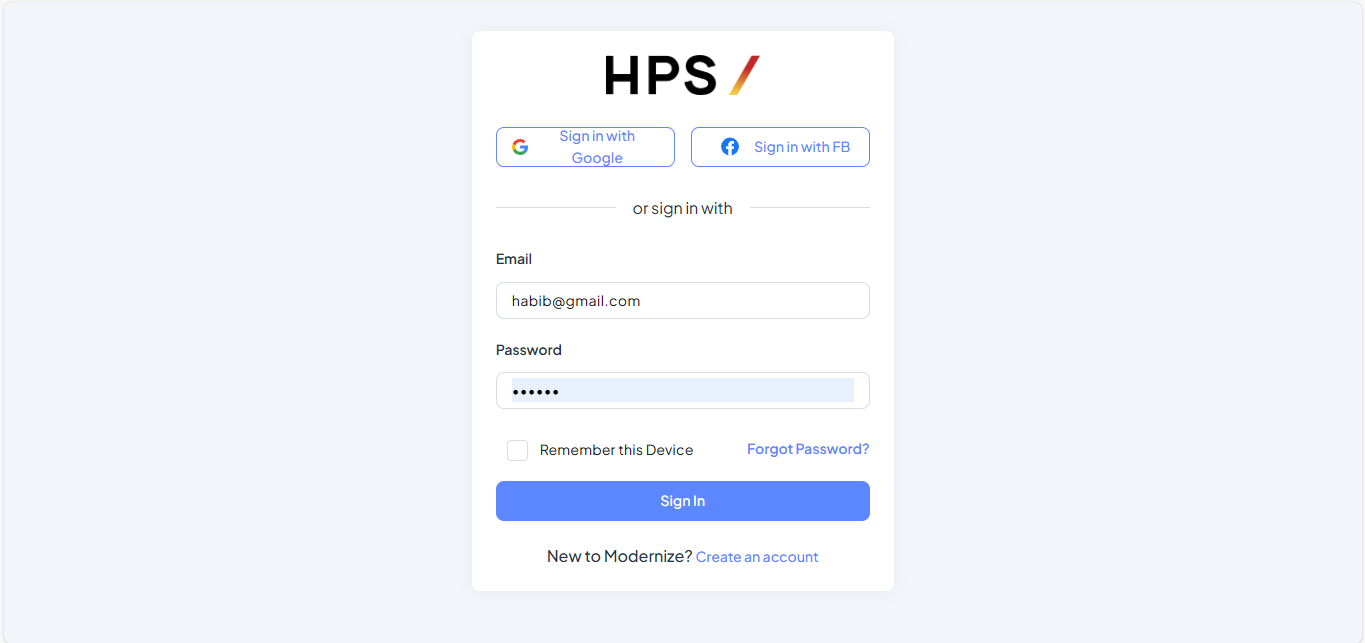
\includegraphics[width=1\textwidth]{figures/images/Auth_SC.png}
\caption{Interface de connexion de l'application HPS}
\label{fig:mobile_app_architecture}
\end{figure}

Cette interface permet aux utilisateurs de se connecter à l'espace sécurisé de l'application \textbf{HPS} en saisissant leur adresse \emph{email} et leur mot de passe.  
L'authentification repose sur un système \textbf{JWT (JSON Web Token)}, avec une gestion des rôles (\texttt{ADMIN} ou \texttt{USER}) permettant de restreindre l'accès à certaines fonctionnalités selon le profil utilisateur.  

De plus, l'interface propose des fonctionnalités supplémentaires telles que :  
\begin{itemize}[label=\textbullet]
    \item \textbf{Récupération de compte} pour les utilisateurs ayant oublié leurs identifiants ;
    \item \textbf{Inscription} pour les nouveaux utilisateurs souhaitant créer un compte.
\end{itemize}


\subsection{Interface d'inscription}


\begin{figure}[H]
\centering
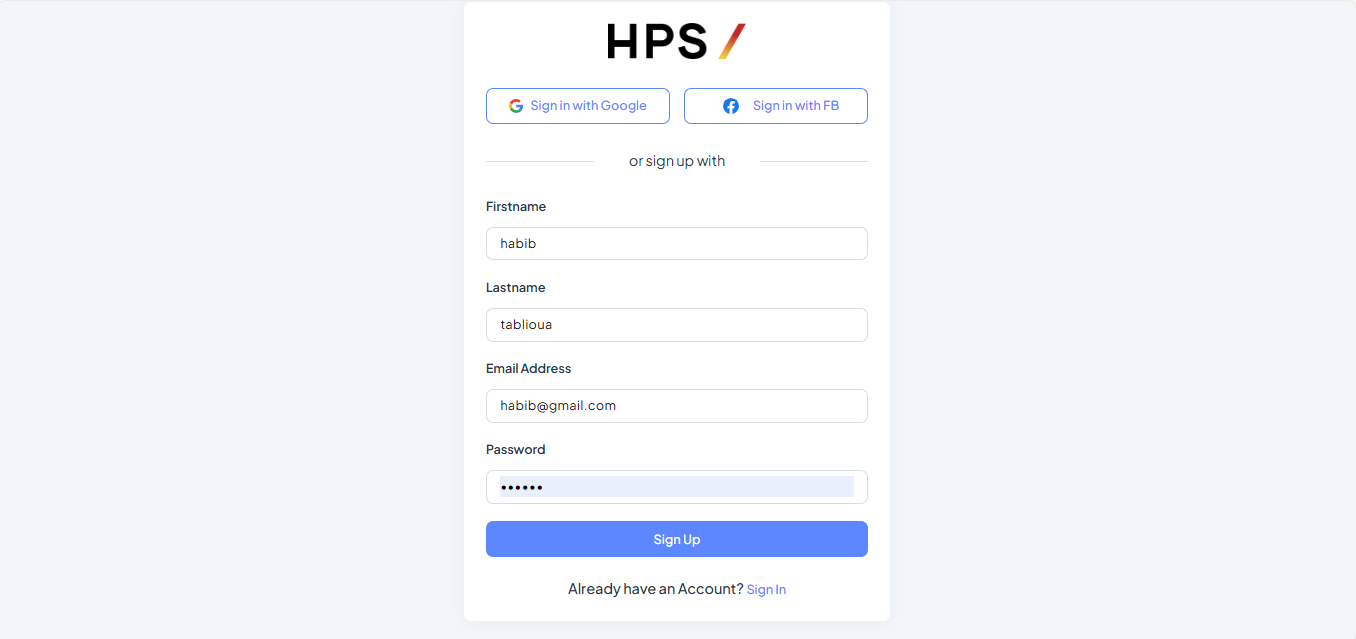
\includegraphics[width=1\textwidth]{figures/images/Inscription_CE.png}
\caption{Interface d'inscription de l'application HPS}
\label{fig:mobile_app_architecture}
\end{figure}

Cette interface permet aux nouveaux utilisateurs de créer un compte dans l'application HPS en saisissant leurs informations personnelles (prénom, nom de famille, adresse email) et en définissant un mot de passe sécurisé. L'interface propose également des options d'inscription alternatives via Google et Facebook pour faciliter le processus d'inscription. Une fois le formulaire complété, l'utilisateur peut accéder à l'espace sécurisé de l'application avec les permissions correspondant à son profil.


\subsection{Menus selon les rôles utilisateurs}

\begin{figure}[H]
    \centering
    \begin{minipage}[b]{0.45\textwidth}
        \centering
        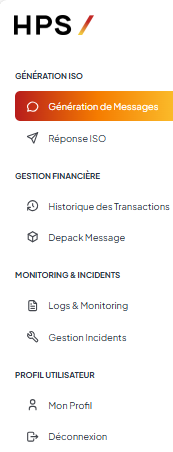
\includegraphics[height=7cm, keepaspectratio]{figures/images/menu_testeur.png}
        \caption{Menus selon les rôles - Interface testeur}
        \label{fig:menu-testeur}
    \end{minipage}
    \hfill
    \begin{minipage}[b]{0.45\textwidth}
        \centering
        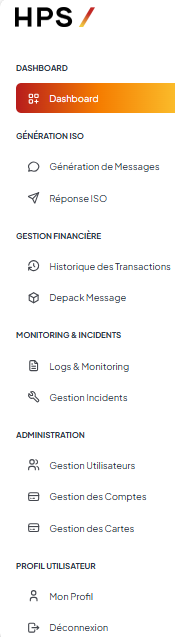
\includegraphics[height=7cm, keepaspectratio]{figures/images/menu_admin.png}
        \caption{Menus selon les rôles - Interface administrateur}
        \label{fig:menu-admin}
    \end{minipage}
\end{figure}


\noindent
Ces figures illustrent la répartition des accès et fonctionnalités de l'application HPS en fonction des rôles attribués aux utilisateurs.

\begin{itemize}[label=\textbullet]
    \item \textbf{Accès communs :} Les administrateurs et testeurs disposent d'un accès aux menus essentiels tels que \textit{Génération de Messages}, \textit{Depacking}, \textit{Historique des Transactions}, \textit{Logs et Monitoring}, et \textit{Gestion des Incidents}, afin d'assurer un suivi global et une analyse en temps réel des activités.
    \item \textbf{Accès restreints :} Les administrateurs seuls ont la responsabilité de la gestion complète des utilisateurs, des comptes et des cartes, assurant ainsi une maîtrise renforcée des éléments sensibles du système financier. Ils accèdent également au \textit{Dashboard} avec des privilèges étendus.
\end{itemize}

Cette organisation hiérarchisée des menus et droits d'accès garantit une navigation fluide, une gestion optimale des ressources et un haut niveau de sécurité au sein de l'application HPS.



\subsection{Interface du tableau de bord}

\begin{figure}[H]
\centering
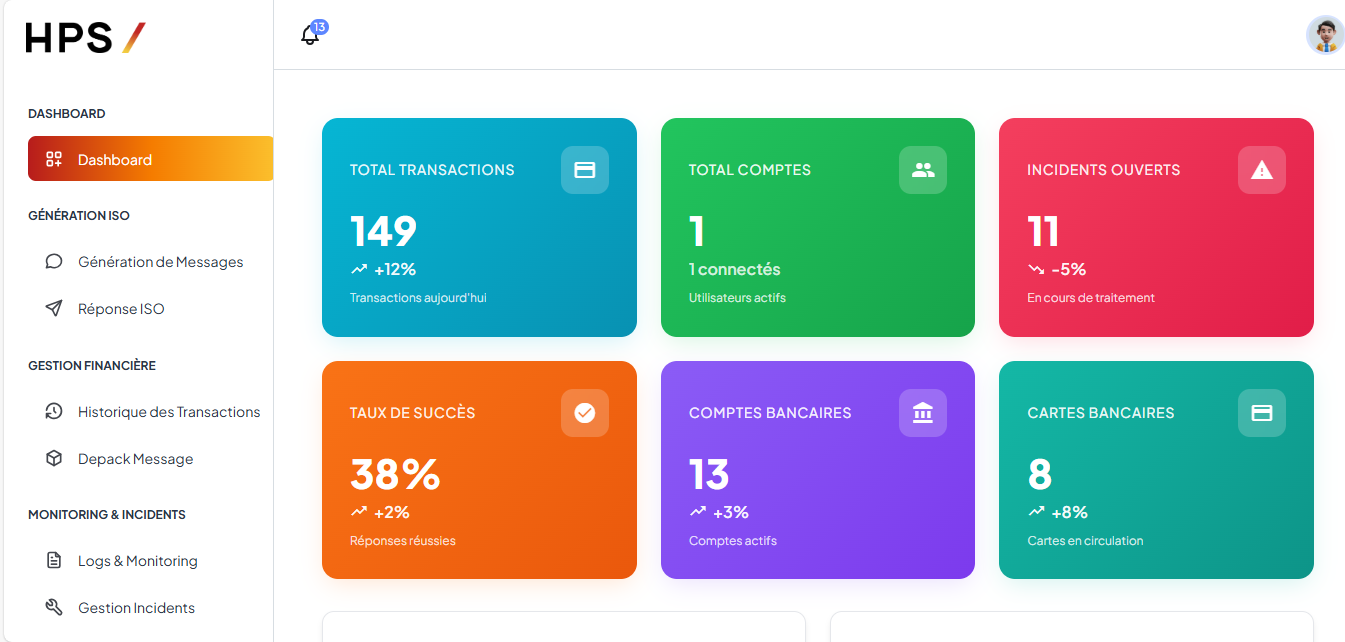
\includegraphics[width=1\textwidth]{figures/images/TableauBord.png}
\caption{Tableau de bord principal de l'application HPS}
\label{fig:mobile_app_architecture}
\end{figure}

\paragraph{} 
Ce tableau de bord présente les principaux indicateurs liés à la gestion des transactions ISO 8583 et au monitoring du système financier. Il regroupe des métriques clés, à la fois quotidiennes et cumulées, permettant un suivi précis et en temps réel de l'activité transactionnelle. Les indicateurs incluent notamment le nombre total de transactions, le taux de succès des réponses ISO, le nombre d'incidents ouverts, ainsi que des informations relatives à la gestion des comptes bancaires et des cartes. Ces données sont représentées sous forme de cartes colorées avec des indicateurs visuels de progression, ce qui facilite l'analyse et la prise de décision opérationnelle.




\subsection{Tableau de bord - Métriques et analyses en temps réel}

\begin{figure}[H]
    \centering
    \begin{minipage}[b]{0.45\textwidth}
        \centering
        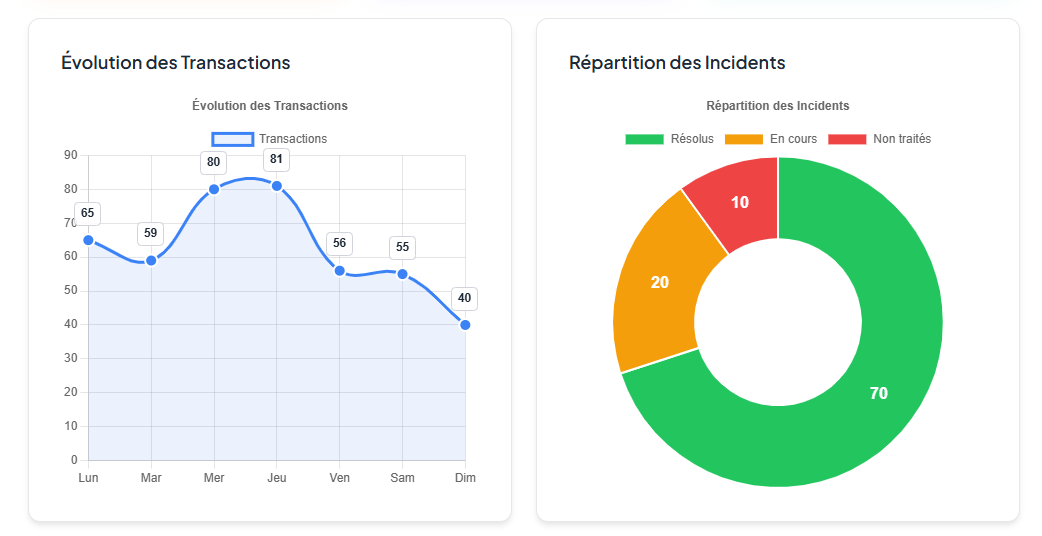
\includegraphics[width=\textwidth]{figures/images/Stat1.png}
    \end{minipage}
    \hfill
    \begin{minipage}[b]{0.45\textwidth}
        \centering
        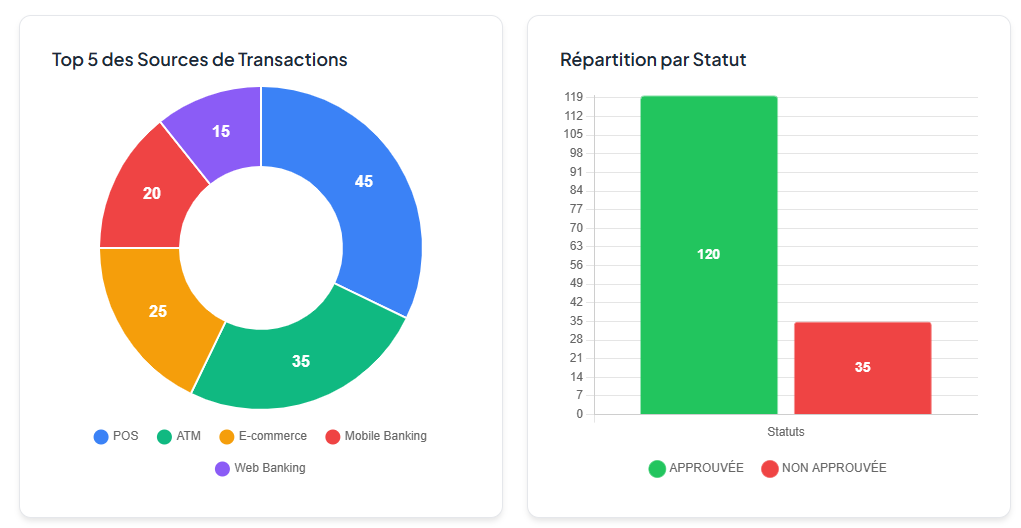
\includegraphics[width=\textwidth]{figures/images/Stat2.png}
    \end{minipage}
    \caption{Métriques et analyses en temps réel}
    \label{fig:metriques-analyses}
\end{figure}

\noindent
Cette figure illustre deux aspects majeurs de l’analyse des transactions dans l’application HPS :

\begin{itemize}[label=\textbullet]
    \item \textbf{Analyse des transactions et répartition des incidents :} 
    Le premier graphique se compose de deux volets complémentaires. D'une part, un graphique linéaire représentant l'évolution hebdomadaire du volume de transactions, utile pour détecter les tendances et les pics d'activité. D'autre part, un diagramme en anneau indiquant la répartition des incidents en trois catégories : \textit{Résolus}, \textit{En cours} et \textit{Non traités}. Cette représentation facilite l'évaluation de l'efficacité du processus de résolution et met en lumière les zones nécessitant une attention particulière.

    \vspace{0.5cm} % <-- Ajoute un espace vertical

    \item \textbf{Répartition des sources et du statut des transactions :} 
    Le second graphique met en évidence la distribution des transactions selon différents canaux (POS, ATM, E-commerce, Mobile Banking, Web Banking), permettant d'identifier les canaux les plus sollicités. En parallèle, il présente la répartition des transactions en fonction de leur statut, distinguant celles qui sont \textit{Approuvées} de celles qui sont \textit{Non approuvées}. Cette double visualisation fournit une vue synthétique sur la performance et la fiabilité des traitements.
\end{itemize}


\subsection{Interface de génération de messages ISO}

\begin{figure}[H]
\centering
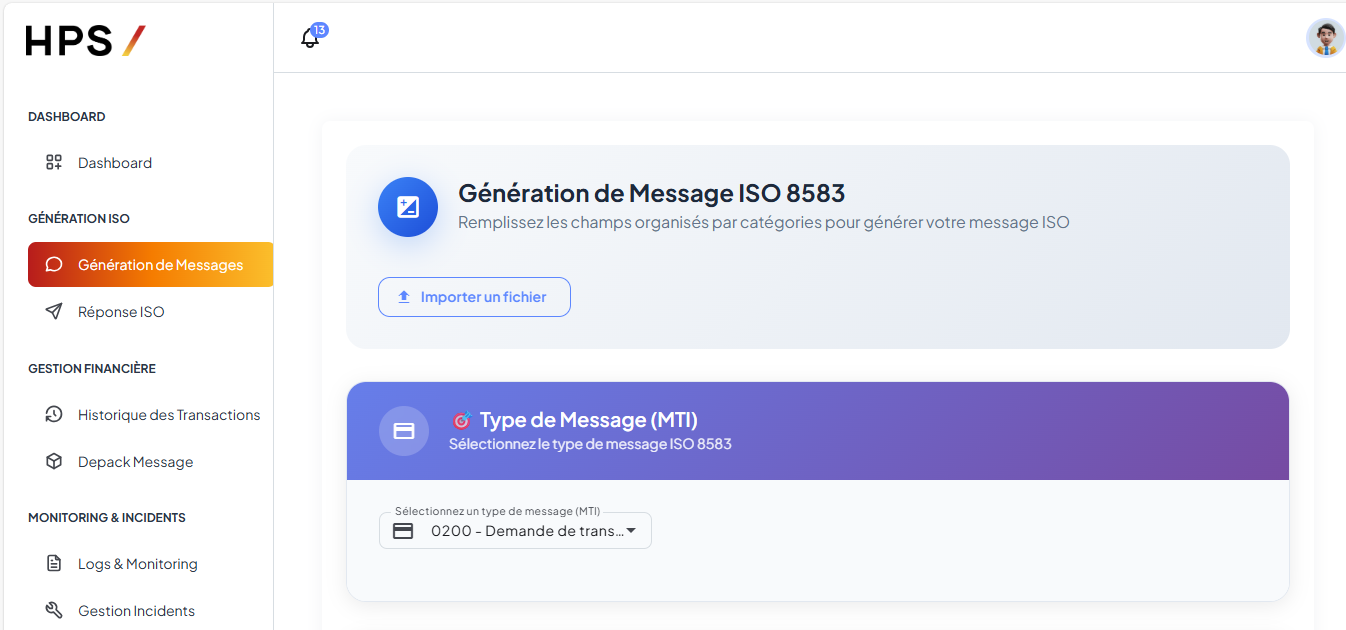
\includegraphics[width=1\textwidth]{figures/images/CE_GenerationMessage}
\caption{Interface de génération de messages ISO}
\label{fig:mobile_app_architecture}
\end{figure}

\paragraph{} 
Cette interface permet aux utilisateurs de générer des messages \textbf{ISO 8583}, standard international pour les transactions financières. 
L'écran principal présente un formulaire complet avec des options d'import de fichiers et de sélection de types de messages prédéfinis. 
Les utilisateurs peuvent soit importer un fichier de configuration existant pour accélérer le processus, soit sélectionner manuellement le type de message souhaité dans un menu déroulant, puis remplir les différents champs selon leurs besoins spécifiques. 

Cette fonctionnalité est essentielle pour tester la communication entre les systèmes de paiement, valider les protocoles de transaction, et assurer la conformité des échanges de données dans l'infrastructure financière.


\begin{enumerate}[label=\alph*)]
\item \textbf{Sélection du type de message (MTI)} \\


\begin{figure}[H]
\centering
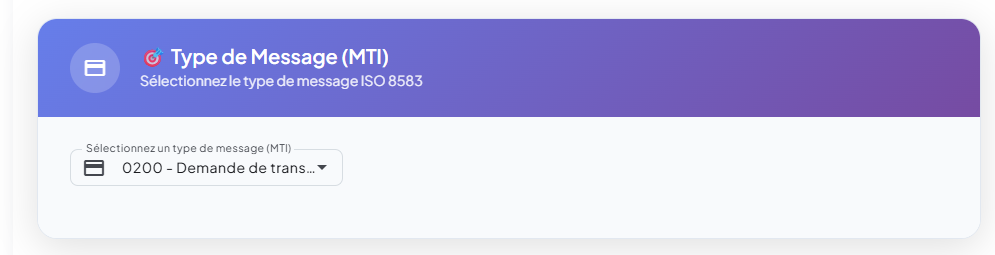
\includegraphics[width=1\textwidth]{figures/images/MTI.png}
\caption{Sélection du MTI}
\label{fig:mobile_app_architecture}
\end{figure}

L'interface présente un menu déroulant avec différents types de messages prédéfinis. Par exemple, le code \texttt{0200} correspond à une \og Demande de transaction \fg{} : c'est le message initial envoyé par un terminal de paiement (\textit{POS, ATM}) pour demander l'autorisation d'une transaction. D'autres codes MTI existent, tels que :

\begin{table}[H]
\centering
\rowcolors{2}{blue!10!white}{white}
\renewcommand{\arraystretch}{1.5}
\begin{tabular}{|>{\bfseries}c|m{10cm}|m{10cm}|}
\hline
\rowcolor{blue!20}
\textbf{Code MTI} & \textbf{Description} \\
\hline
0200 & Demande de transaction(\textit{Transaction Request}) \\
\hline
0210 & Réponse d'autorisation (\textit{Authorization Response}) \\
\hline
0220 & Demande de conseil (\textit{Advice Request}) \\
\hline
0230 & Réponse de conseil (\textit{Advice Response}) \\
\hline
0400 & Demande de remboursement (\textit{Reversal Request}) \\
\hline
0410 & Réponse de remboursement (\textit{Reversal Response}) \\
\hline
0420 & Demande de compensation (\textit{Settlement Request}) \\
\hline
0430 & Réponse de compensation (\textit{Settlement Response}) \\
\hline
0800 & Demande de gestion réseau (\textit{Network Management Request}) \\
\hline
0810 & Réponse de gestion réseau (\textit{Network Management Response}) \\
\hline
\end{tabular}
\caption{\textbf{Codes MTI ISO 8583 et leurs significations}}
\label{tab:mti-codes}
\end{table}



Cette sélection est \textbf{cruciale} car elle détermine automatiquement quels champs de données seront obligatoires et lesquels seront optionnels dans le message final. Elle permet également de s'assurer que le message généré respecte la structure attendue par le système de traitement des transactions financières.

 \vspace{0.5cm} % <-- Ajoute un espace vertical

\item \textbf{Informations de base du message ISO} \\


\begin{figure}[H]
\centering
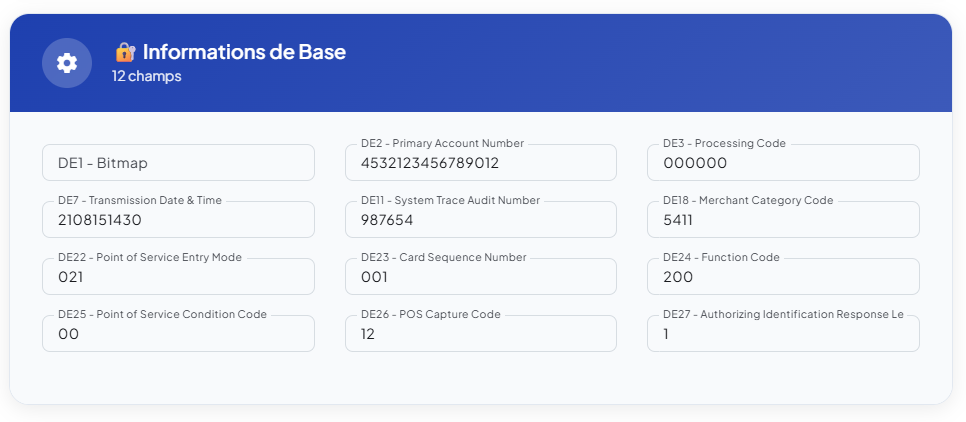
\includegraphics[width=1\textwidth]{figures/images/InformationsBase.png}
\caption{Saisie des informations de base du message ISO}
\label{fig:mobile_app_architecture}
\end{figure}

Cette section de l'interface de génération de messages ISO est dédiée à la saisie des informations fondamentales de la transaction. Elle regroupe \textbf{12 champs essentiels} qui définissent les caractéristiques principales de l'opération financière. Ces champs sont cruciaux pour construire un message \textbf{ISO 8583} valide et représentatif d'une transaction réelle, permettant ainsi de tester divers scénarios.

Chaque champ est présenté avec son identifiant, son libellé et un champ de saisie pour la valeur correspondante :

\begin{itemize}[label=\textbullet]
    \item \textbf{Champ 1 - Bitmap :} Ce champ binaire indique la présence des autres champs dans le message. Il est généralement généré automatiquement en fonction des champs renseignés.
    \item \textbf{Champ 2 - Primary Account Number (PAN) :} Représente le numéro de compte principal, typiquement le numéro de carte bancaire.
    \item \textbf{Champ 3 - Processing Code :} Définit le type de transaction (\textit{achat, retrait, remboursement}) et les comptes impliqués.
    \item \textbf{Champ 7 - Transmission Date \& Time :} Indique la date et l'heure de la transmission du message.
    \item \textbf{Champ 11 - System Trace Audit Number (STAN) :} Numéro unique attribué par le système d'origine pour identifier la transaction.
    \item \textbf{Champ 18 - Merchant Category Code (MCC) :} Identifie le type d'activité du commerçant.
    \item \textbf{Champ 22 - Point of Service Entry Mode :} Décrit la méthode de capture des données de la carte au point de vente.
    \item \textbf{Champ 23 - Card Sequence Number :} Numéro de séquence de la carte, utilisé lorsque plusieurs cartes sont émises pour le même compte.
    \item \textbf{Champ 24 - Function Code :} Spécifie la fonction du message au sein d'un réseau particulier.
    \item \textbf{Champ 25 - Point of Service Condition Code :} Décrit les conditions spécifiques de la transaction au point de vente.
    \item \textbf{Champ 26 - POS Capture Code :} Indique la capacité du terminal de point de vente à capturer les données de la carte.
    \item \textbf{Champ 27 - Authorizing Identification Response Length :} La longueur de la réponse d'identification d'autorisation.
\end{itemize}

\item \textbf{ Montants et frais de transaction} \\

\begin{figure}[H]
\centering
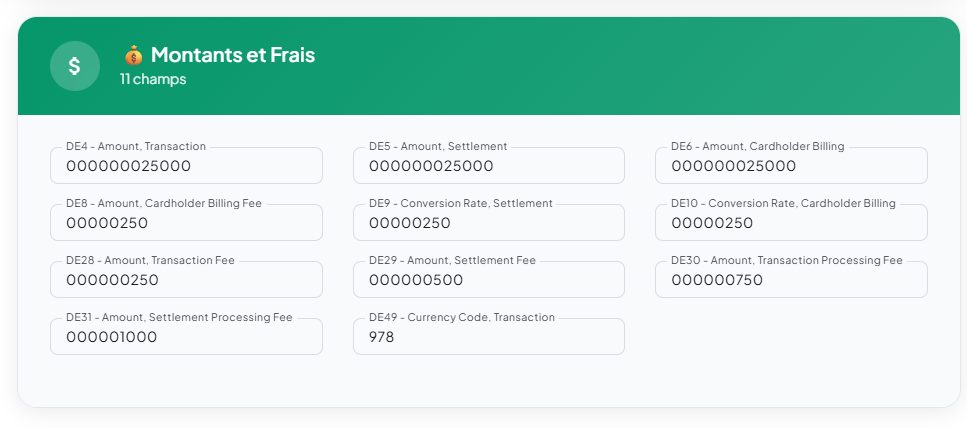
\includegraphics[width=1\textwidth]{figures/images/MontantFrais.png}
\caption{Saisie des montants et frais pour un message ISO}
\label{fig:mobile_app_architecture}
\end{figure}

Cette section de l'interface de génération de messages ISO est dédiée à la saisie des informations financières de la transaction. Elle regroupe \textbf{11 champs essentiels} qui définissent les montants, les frais et les taux de conversion associés à l'opération financière. Ces champs sont cruciaux pour construire un message \textbf{ISO 8583} précis et représentatif d'une transaction réelle.

Chaque champ est présenté avec son identifiant, son libellé et un champ de saisie pour la valeur correspondante :

\begin{table}[H]
\centering
\rowcolors{2}{blue!10!white}{white}
\renewcommand{\arraystretch}{1.5}
\begin{tabular}{|>{\bfseries}c|m{8cm}|m{6cm}|}
\hline
\rowcolor{blue!20}
\textbf{Champ} & \textbf{Nom} & \textbf{Description} \\
\hline
4 & Amount, Transaction & Montant principal de la transaction (ex : 250,00). \\
\hline
5 & Amount, Settlement & Montant de la compensation, généralement identique au montant de la transaction. \\
\hline
6 & Amount, Cardholder Billing & Montant facturé au porteur de la carte, qui peut inclure des frais. \\
\hline
8 & Amount, Cardholder Billing Fee & Frais facturés au porteur de la carte. \\
\hline
9 & Conversion Rate, Settlement & Taux de conversion utilisé pour la compensation. \\
\hline
10 & Conversion Rate, Cardholder Billing & Taux de conversion appliqué au porteur de la carte. \\
\hline
28 & Amount, Transaction Fee & Frais de transaction. \\
\hline
29 & Amount, Settlement Fee & Frais de compensation. \\
\hline
30 & Amount, Transaction Processing Fee & Frais de traitement de la transaction. \\
\hline
31 & Amount, Settlement Processing Fee & Frais de traitement de la compensation. \\
\hline
49 & Currency Code, Transaction & Code de la devise de la transaction (ex : 978 pour l'Euro). \\
\hline
\end{tabular}
\caption{Champs financiers ISO 8583 - Montants et frais de transaction}
\label{tab:iso-finance-fields}
\end{table}


\item \textbf{Dates et heures de transaction} \\

\begin{figure}[H]
\centering
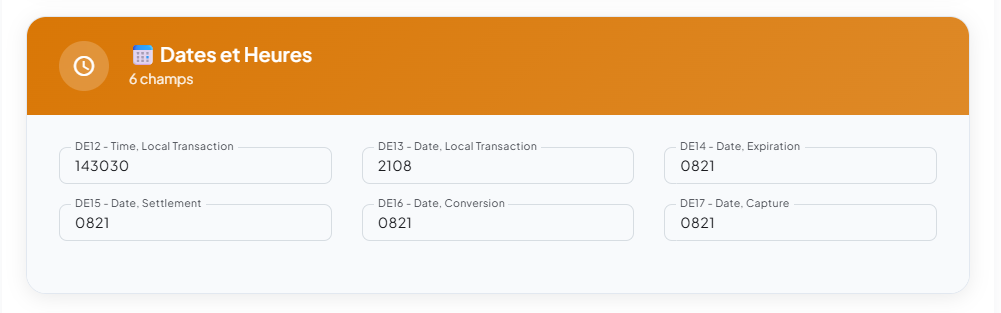
\includegraphics[width=1\textwidth]{figures/images/DateHeure.png}
\caption{Saisie des dates et heures de transaction ISO}
\label{fig:mobile_app_architecture}
\end{figure}

Cette section de l'interface de génération de messages ISO 8583 est dédiée à la saisie des informations temporelles cruciales pour chaque transaction. Elle regroupe six champs essentiels qui définissent les différents moments clés de l'opération financière, permettant un suivi précis et une traçabilité complète. Ces champs sont indispensables pour la validation, la réconciliation et l'archivage des transactions ISO 8583.

Chaque champ est présenté avec son identifiant, son libellé et un champ de saisie pour la valeur correspondante :

\begin{itemize}[label=\textbullet]
    \item \textbf{Champ 12 - Time, Local Transaction} : Indique l'heure locale à laquelle la transaction a été initiée (\textit{format HHMMSS}).
    
    \item \textbf{Champ 13 - Date, Local Transaction} : Spécifie la date locale à laquelle la transaction a été initiée (\textit{format MMDD}).
    
    \item \textbf{Champ 14 - Date, Expiration} : Représente la date d'expiration d'une carte ou d'un instrument de paiement utilisé pour la transaction (\textit{format MMYY}).
    
    \item \textbf{Champ 15 - Date, Settlement} : Indique la date à laquelle la transaction est prévue pour être réglée ou compensée entre les institutions financières (\textit{format MMDD}).
    
    \item \textbf{Champ 16 - Date, Conversion} : Spécifie la date à laquelle une conversion de devise a eu lieu, si applicable (\textit{format MMDD}).
    
    \item \textbf{Champ 17 - Date, Capture} : Représente la date à laquelle la transaction a été capturée ou traitée par le système (\textit{format MMDD}).
\end{itemize}


\item \textbf{ Informations institutionnelles} \\

Cette section de l'interface de génération de messages ISO est dédiée à la saisie des informations relatives aux institutions financières impliquées dans la transaction. Elle regroupe cinq champs essentiels qui permettent d'identifier l'origine et le cheminement du message, assurant ainsi la traçabilité et la conformité des opérations. Ces champs sont cruciaux pour les processus d'autorisation, de compensation et de règlement.

Chaque champ est présenté avec son identifiant, son libellé et un champ de saisie pour la valeur correspondante :

\begin{table}[H]
\centering
\rowcolors{2}{blue!10!white}{white}
\renewcommand{\arraystretch}{1.5}
\begin{tabular}{|>{\bfseries}c|m{4cm}|m{7cm}|}
\hline
\rowcolor{blue!20}
\textbf{Champ} & \textbf{Nom} & \textbf{Description} \\
\hline
19 & Acquiring Institution Country Code & Code pays de l'institution acquéreuse, c'est-à-dire la banque ou l'entité qui a initié la transaction. \\
\hline
20 & PAN Extended Country Code & Code pays étendu du numéro de compte principal (PAN), souvent lié au pays d'émission de la carte. \\
\hline
21 & Forwarding Institution Country Code & Code pays de l'institution émettrice, c'est-à-dire la banque ou l'entité qui a transmis le message pour traitement. \\
\hline
32 & Acquiring Institution ID Code & Code d'identification unique de l'institution acquéreuse. \\
\hline
33 & Forwarding Institution ID Code & Code d'identification unique de l'institution émettrice. \\
\hline
\end{tabular}
\caption{Champs ISO 8583 - Informations institutionnelles}
\label{tab:iso-institution-fields}
\end{table}

Cette section de l'interface de génération de messages ISO est dédiée à la saisie des informations spécifiques à la carte bancaire utilisée pour la transaction. Elle regroupe des champs essentiels qui permettent d'identifier la carte et de simuler les données lues depuis une piste magnétique. Ces informations sont cruciales pour les transactions impliquant des cartes de paiement et sont utilisées pour l'autorisation et le traitement des opérations.

Chaque champ est présenté avec son identifiant, son libellé et un champ de saisie pour la valeur correspondante :

\begin{itemize}[label=\textbullet]
    \item \textbf{Champ 34 - Primary Account Number, Extended} : Ce champ contient le numéro de compte principal étendu (\textit{PAN}), qui est l'identifiant unique de la carte. Il est utilisé pour identifier le compte du titulaire de la carte.
    
    \item \textbf{Champ 35 - Track 2 Data} : Ce champ contient les données de la piste 2 de la carte magnétique, qui incluent généralement le PAN, la date d'expiration et le code de service. Ces données sont lues par les terminaux de paiement.
    
    \item \textbf{Champ 36 - Track 3 Data} : Ce champ contient les données de la piste 3 de la carte magnétique. Cette piste est moins couramment utilisée que les pistes 1 et 2, mais peut contenir des informations supplémentaires spécifiques à l'émetteur ou à l'application.
    
    \item \textbf{Champ 45 - Track 1 Data} : Ce champ contient les données de la piste 1 de la carte magnétique, qui incluent le PAN, le nom du titulaire de la carte, la date d'expiration et le code de service. Ces données sont également lues par les terminaux.
\end{itemize}


\item \textbf{ Informations du commerce} \\

\begin{figure}[H]
\centering
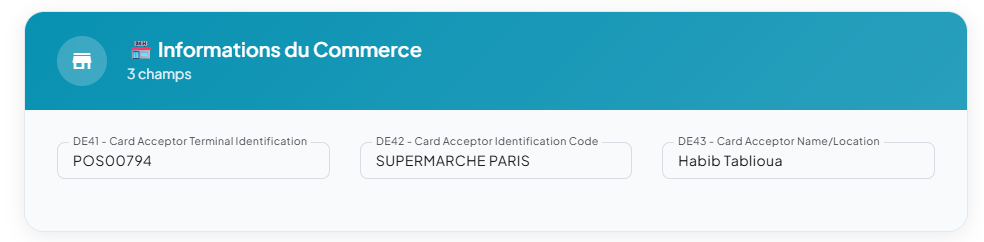
\includegraphics[width=1\textwidth]{figures/images/Commerce.png}
\caption{Saisie des informations du commerçant}
\label{fig:mobile_app_architecture}
\end{figure}

Cette section de l'interface de génération de messages ISO est dédiée à la saisie des informations relatives au \textbf{commerçant (point de vente)} où la transaction a eu lieu. Elle regroupe trois champs essentiels permettant d'identifier le terminal, le code du commerçant et le nom/lieu du commerçant. Ces informations sont fondamentales pour :
\begin{itemize}[label=\textbullet]
    \item la traçabilité des transactions.
    \item la détection de fraudes.
    \item la réconciliation des paiements.
\end{itemize}

Chaque champ est présenté avec son identifiant, son libellé et un champ de saisie pour la valeur correspondante :

\begin{itemize}[label=\textbullet]
    \item \textbf{Champ 41 - Card Acceptor Terminal Identification} : Ce champ identifie de manière unique le terminal de paiement (POS, ATM, etc.) où la transaction a été initiée.
    \item \textbf{Champ 42 - Card Acceptor Identification Code} : Ce code identifie le commerçant ou l'établissement acceptant la carte. Il est souvent attribué par l'acquéreur et permet de regrouper les transactions d'un même commerçant.
    \item \textbf{Champ 43 - Card Acceptor Name/Location} : Ce champ fournit le nom et l'emplacement géographique du commerçant. Il est utilisé pour afficher des informations claires sur les relevés de compte des titulaires de carte.
\end{itemize}

\item \textbf{ Données Supplémentaires} \\

\begin{figure}[H]
\centering
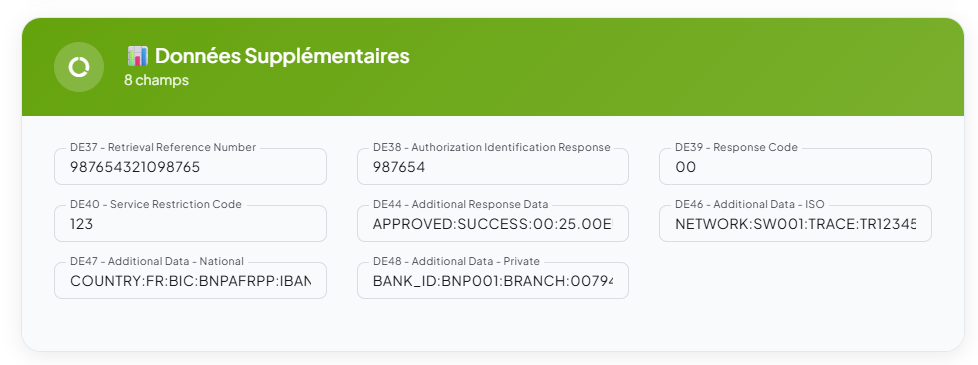
\includegraphics[width=1\textwidth]{figures/images/DonneeSup.png}
\caption{Saisie des données supplémentaires du message ISO}
\label{fig:mobile_app_architecture}
\end{figure}

Cette section de l'interface de génération de messages ISO est dédiée à la saisie et à l'affichage de données additionnelles qui complètent les informations principales d'une transaction. Elle regroupe huit champs essentiels qui fournissent des détails spécifiques sur la référence de la transaction, la réponse d'autorisation, les codes de service, ainsi que des informations supplémentaires au niveau de la réponse, de la norme ISO, national et privé. Ces données sont cruciales pour une traçabilité approfondie, l'audit et la compréhension contextuelle des opérations financières.

Chaque champ est présenté avec son identifiant, son libellé et un champ de saisie pour la valeur correspondante :

\begin{table}[H]
\centering
\rowcolors{2}{blue!10!white}{white}
\renewcommand{\arraystretch}{1.5}
\begin{tabular}{|>{\bfseries}c|m{7cm}|m{7cm}|}
\hline
\rowcolor{blue!20}
\textbf{Champ} & \textbf{Nom} & \textbf{Description} \\
\hline
37 & Retrieval Reference Number & Numéro de référence unique attribué à la transaction pour son suivi. \\
\hline
38 & Authorization Identification Response & Code d'identification de l'autorisation de la transaction. \\
\hline
39 & Response Code & Code indiquant le statut de la réponse de la transaction (succès, échec, etc.). \\
\hline
40 & Service Restriction Code & Code spécifiant d'éventuelles restrictions de service. \\
\hline
44 & Additional Response Data & Données supplémentaires fournies dans la réponse, souvent pour des détails sur le succès ou l'échec. \\
\hline
46 & Additional Data - ISO & Données additionnelles conformes à la norme ISO. \\
\hline
47 & Additional Data - National & Données supplémentaires spécifiques aux exigences nationales. \\
\hline
48 & Additional Data - Private & Données privées ou spécifiques à l'institution. \\
\hline
\end{tabular}
\caption{Champs ISO 8583 - Données Supplémentaires}
\label{tab:iso-additional-data-fields}
\end{table}


\end{enumerate}




\subsection{Message ISO Généré}

\begin{figure}[H]
\centering
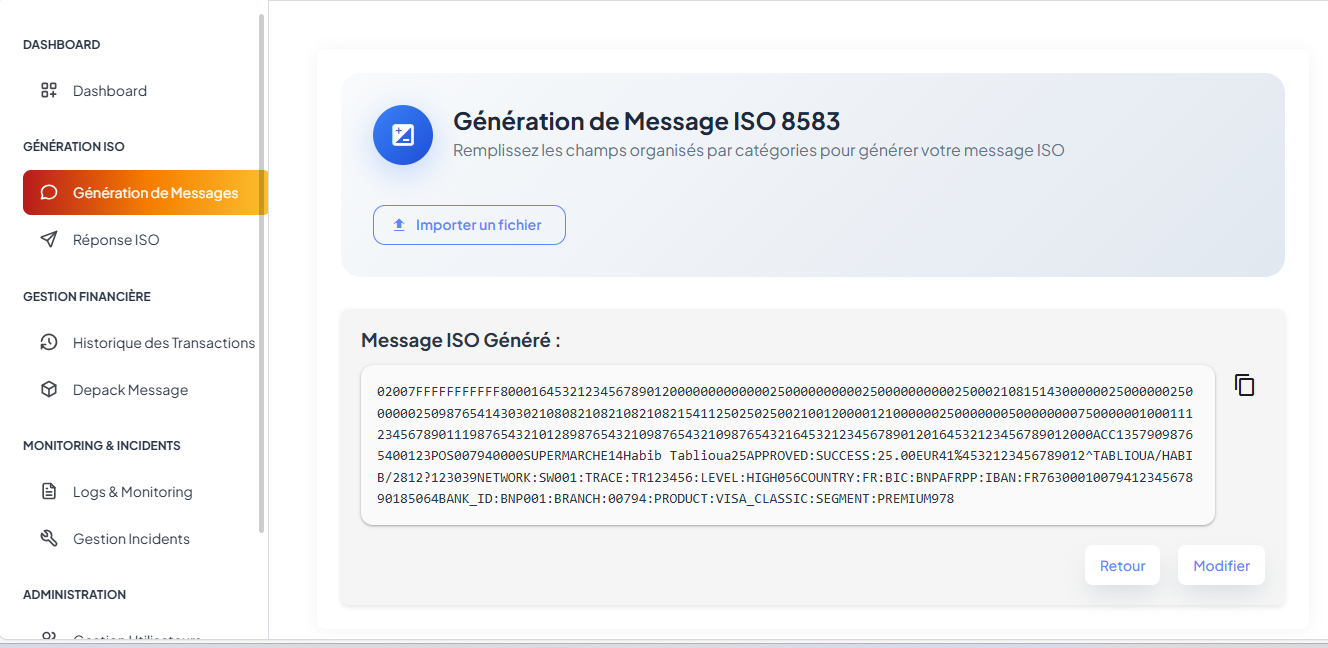
\includegraphics[width=0.9\textwidth]{figures/images/Message.png}
\caption{Interface d'affichage du message ISO 8583 généré}
\label{fig:mobile_app_architecture}
\end{figure}


Cette interface affiche le message \textbf{ISO 8583} complet et formaté, tel qu'il a été construit à partir des champs renseignés par l'utilisateur. 

Ce message est présenté sous sa \textit{forme brute}, une séquence de caractères alphanumériques, représentant l'encodage standardisé de la transaction financière.

Cette visualisation est essentielle pour la vérification et le débogage, permettant aux utilisateurs de s'assurer que le message généré correspond aux spécifications attendues avant son envoi ou son traitement.

\subsection{Interface de dépaquetage de messages ISO}

\begin{figure}[H]
\centering
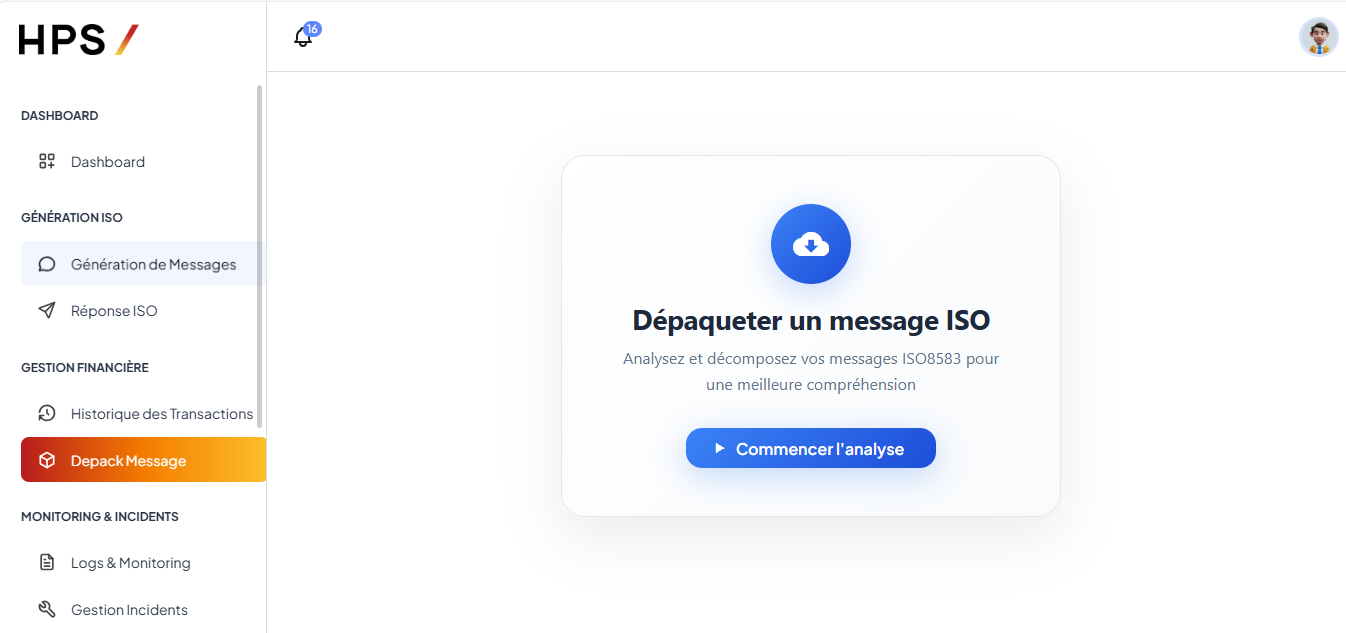
\includegraphics[width=0.9\textwidth]{figures/images/Depack.png}
\caption{Interface de dépaquetage de messages ISO}
\label{fig:mobile_app_architecture}
\end{figure}

Cette interface est dédiée au \textbf{dépaquetage (unpacking)} des messages \textbf{ISO 8583}, un standard international utilisé pour les transactions financières. Elle permet aux utilisateurs d'analyser et de décomposer des messages ISO bruts afin d'en extraire les différents champs de données pour une meilleure compréhension et un débogage facilité.

\begin{enumerate}[label=\alph*)]
\item \textbf{Saisie et analyse du message ISO} \\


\begin{figure}[H]
\centering
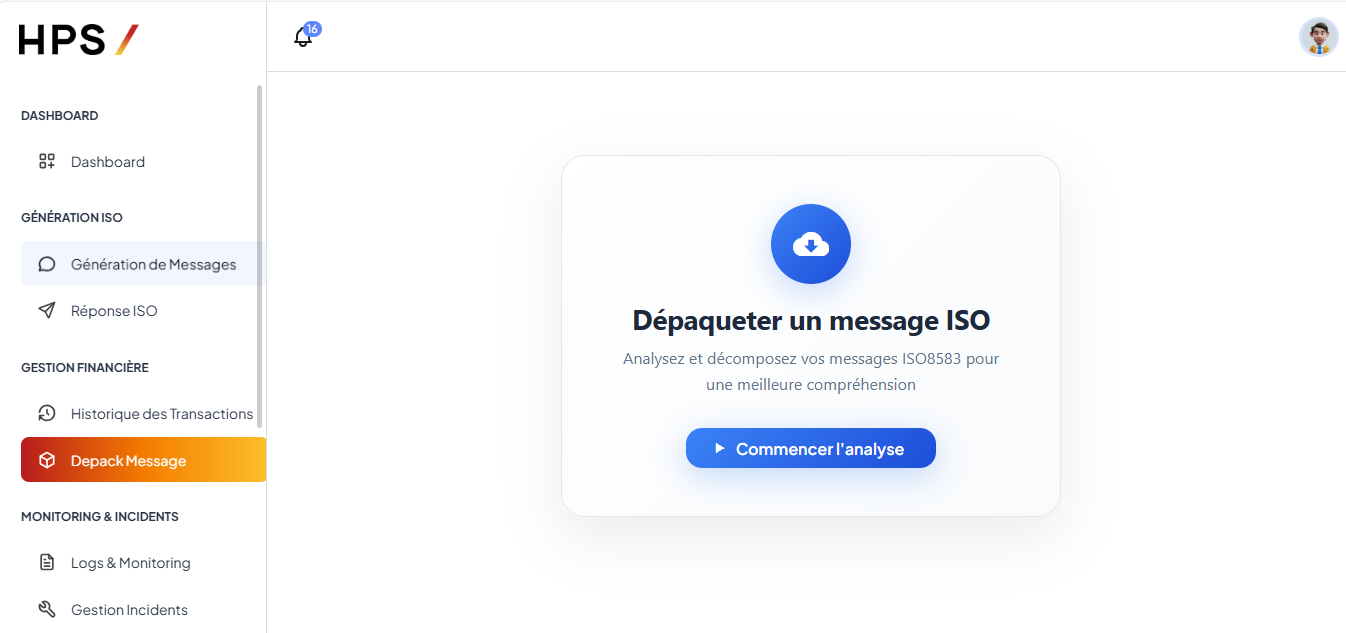
\includegraphics[width=0.9\textwidth]{figures/images/Depack.png}
\caption{Interface de dépaquetage de messages ISO}
\label{fig:mobile_app_architecture}
\end{figure}

Cette section est la partie principale du module de \textbf{dépaquetage de messages ISO 8583}. Elle permet aux utilisateurs de coller un message ISO brut et d'en analyser la structure détaillée. L'objectif est de transformer une séquence de caractères complexe en une représentation lisible et structurée des différents champs de données.

\item \textbf{ Résultats de l'analyse du message ISO} \\


\begin{figure}[H]
    \centering
    \begin{minipage}[b]{0.45\textwidth}
        \centering
        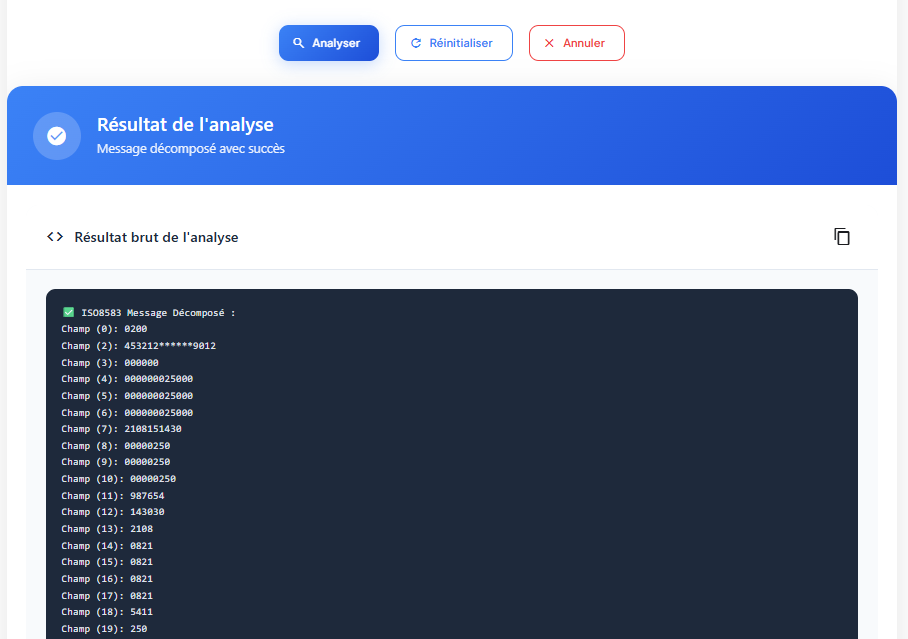
\includegraphics[width=\textwidth]{figures/images/Analyse1.png}
    \end{minipage}
    \hfill
    \begin{minipage}[b]{0.45\textwidth}
        \centering
        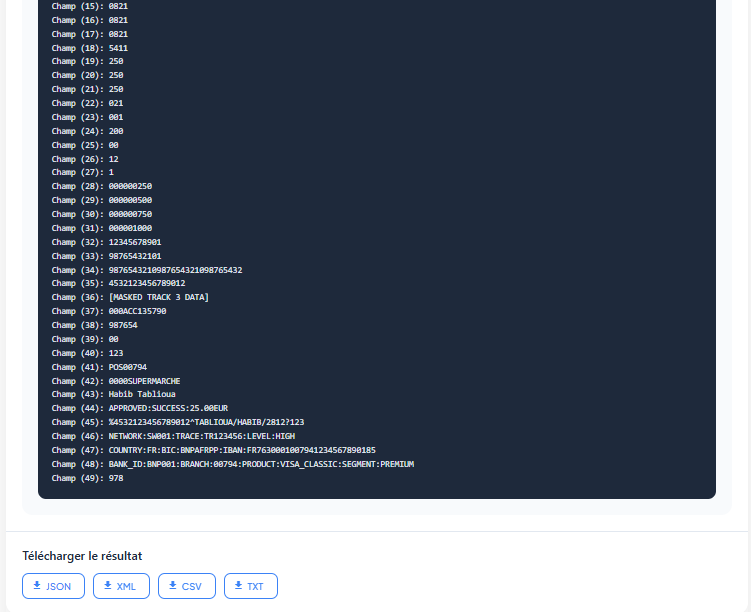
\includegraphics[width=\textwidth]{figures/images/Analyse2.png}
    \end{minipage}
    \caption{Affichage des résultats de l'analyse d'un message ISO 8583}
    \label{fig:metriques-analyses}
\end{figure}

Cette section affiche les résultats obtenus après avoir cliqué sur le bouton \textbf{« Analyser »}. 
Elle présente le message ISO 8583 décomposé et structuré, transformant la séquence de caractères brute en une représentation lisible et organisée des différents champs de données.

\medskip

En bas de l'interface, sous le titre \textbf{« Télécharger le résultat »}, quatre boutons sont disponibles pour exporter les données de l'analyse dans différents formats : \textbf{JSON}, \textbf{XML}, \textbf{CSV} et \textbf{TXT}.

\end{enumerate}

\subsection{Interface d'historique et de gestion des réponses ISO}

\begin{figure}[H]
\centering
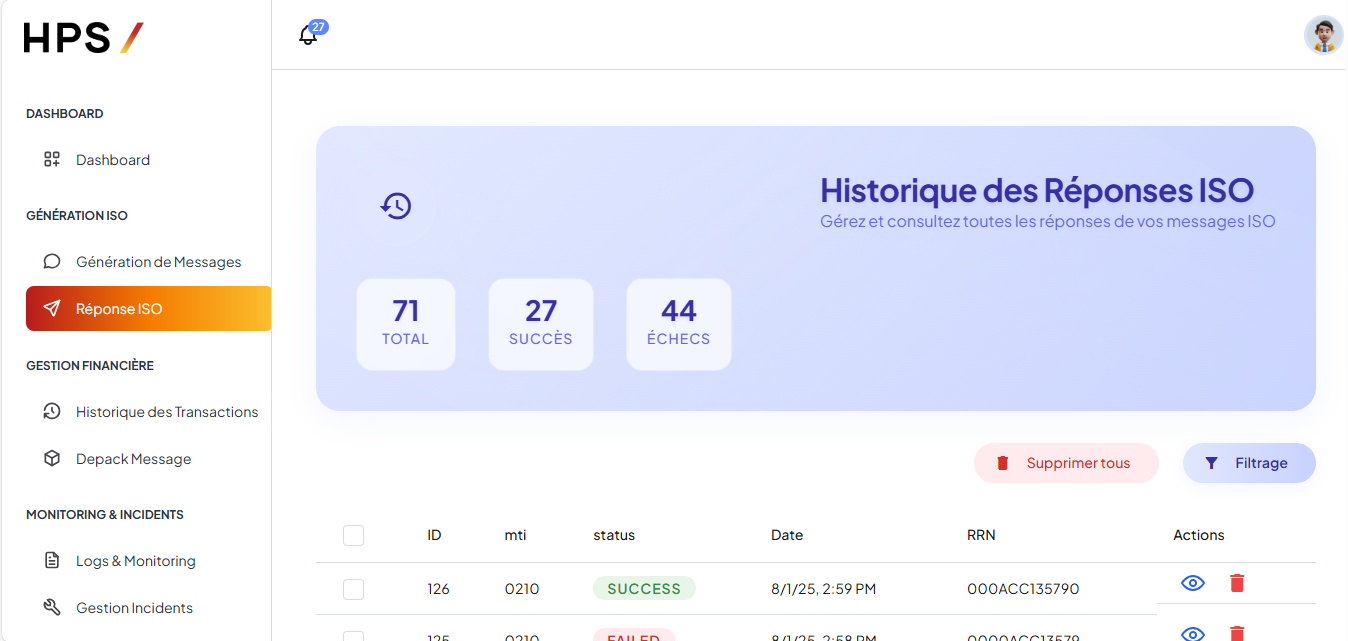
\includegraphics[width=0.9\textwidth]{figures/images/Réponse.png}
\caption{Interface d'historique et de gestion des réponses ISO}
\label{fig:mobile_app_architecture}
\end{figure}

Cette interface est dédiée à la consultation et à la gestion de l'historique des réponses aux messages ISO 8583 envoyés. Elle offre une vue d'ensemble des transactions et permet aux utilisateurs de suivre l'état de chaque réponse, facilitant ainsi le monitoring et le débogage des flux financiers.

L'objectif principal de cette interface est de permettre aux utilisateurs de vérifier si une transaction a été approuvée ou non. En cas d'échec, elle permet de détecter la cause de l'erreur, d'identifier son emplacement précis dans le processus de traitement et de proposer des solutions appropriées. 

Cette fonctionnalité est cruciale pour le diagnostic des problèmes, la résolution des incidents et l'amélioration continue de la performance du système de paiement.

\begin{enumerate}[label=\alph*)]
\item \textbf{Fenêtre modale de détail d'une réponse approuvée} \\

\begin{figure}[H]
\centering
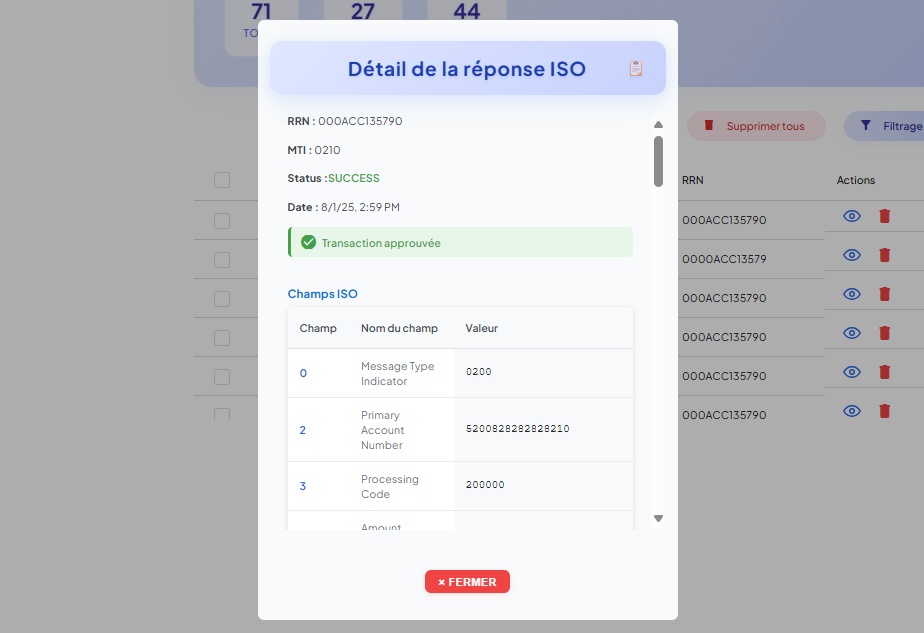
\includegraphics[width=0.9\textwidth]{figures/images/Aprouve.png}
\caption{Interface d'historique et de gestion des réponses approuvée}
\label{fig:mobile_app_architecture}
\end{figure}

Cette fenêtre modale (\textit{pop-up}) s'affiche après avoir cliqué sur le bouton \og Détails \fg{} d'une réponse ISO dans l'historique des transactions. Elle permet d'afficher les informations détaillées d'une réponse spécifique, offrant ainsi une vue complète et structurée des données de la transaction.

\item \textbf{Fenêtres modale de détail d'une réponse non approuvées} \\


\begin{figure}[H]
\centering
\begin{minipage}{0.48\textwidth}
  \centering
  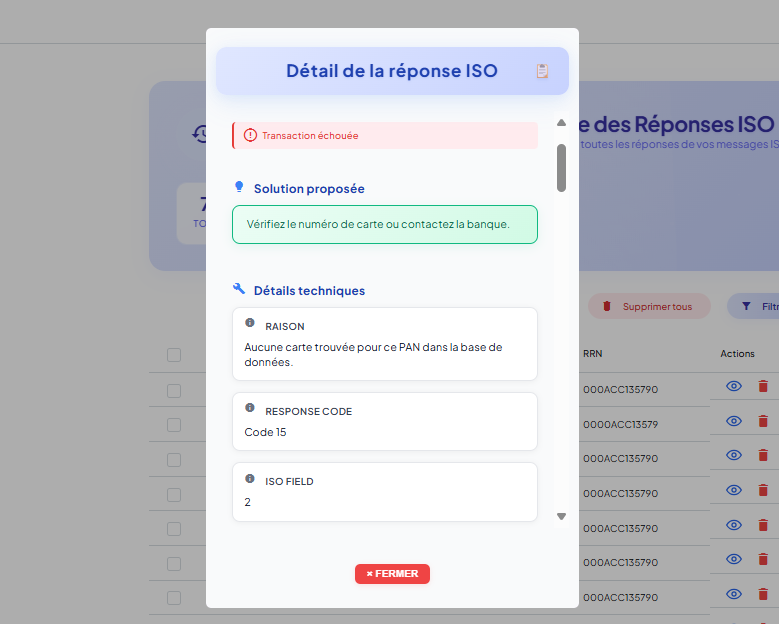
\includegraphics[width=\linewidth]{figures/images/Reponse1.png}
  \captionof{figure}{(a) Fenêtre modale - Code 57}
  \label{fig:reponse3}
\end{minipage}\hfill
\begin{minipage}{0.48\textwidth}
  \centering
  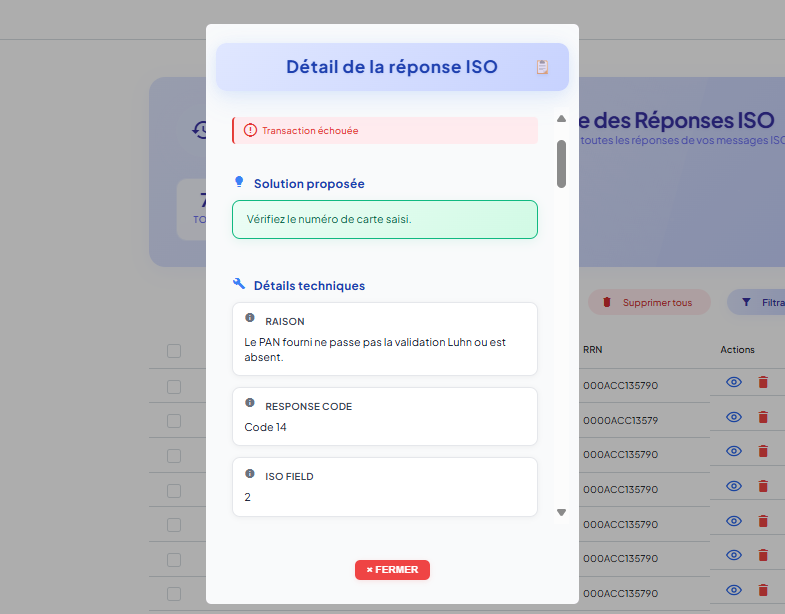
\includegraphics[width=\linewidth]{figures/images/Reponse2.png}
  \captionof{figure}{(a) Fenêtre modale - Code 75(b)}
  \label{fig:reponse4}
\end{minipage}
\end{figure}


\begin{figure}[H]
\centering
\begin{minipage}{0.48\textwidth}
  \centering
  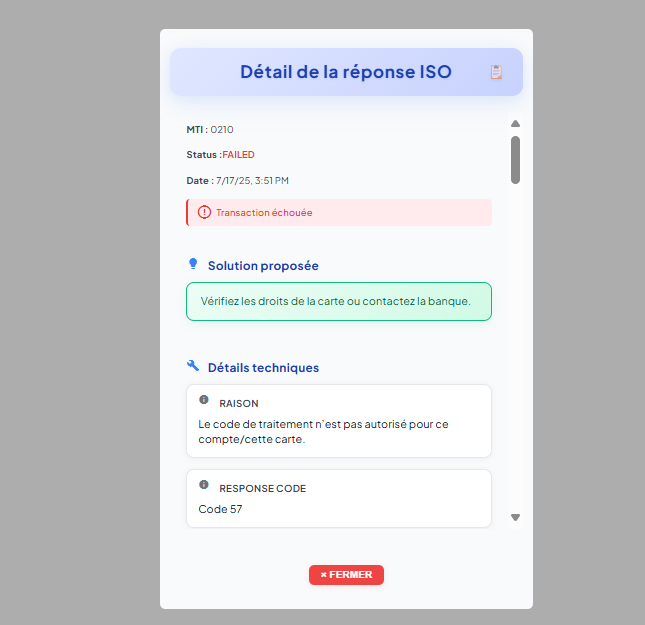
\includegraphics[width=\linewidth]{figures/images/Reponse3.png}
  \captionof{figure}{(c) Fenêtre modale - Code 15}
  \label{fig:reponse3}
\end{minipage}\hfill
\begin{minipage}{0.48\textwidth}
  \centering
  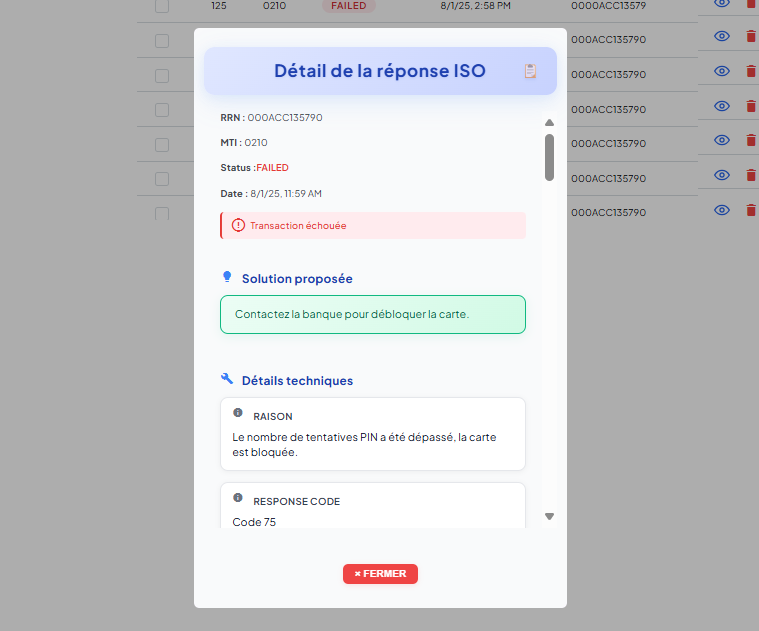
\includegraphics[width=\linewidth]{figures/images/Reponse4.png}
  \captionof{figure}{(d) Fenêtre modale - Code 14}
  \label{fig:reponse4}
\end{minipage}
\end{figure}


\paragraph{}Ces fenêtres modales (a), (b), (c) et (d) permettent d'afficher les informations détaillées d'une réponse spécifique, offrant ainsi une vue complète et structurée des données de la transaction. La section \textit{Détails techniques} fournit des informations précises sur la cause de l'échec : la raison, le code de réponse et le champ ISO concerné. Ces détails permettent aux utilisateurs d'identifier rapidement la source du problème et de prendre les mesures appropriées.
\label{fig:fenetres_modales}

\end{enumerate}


\subsection{Interface d'historique des transactions}
\begin{figure}[H]
\centering
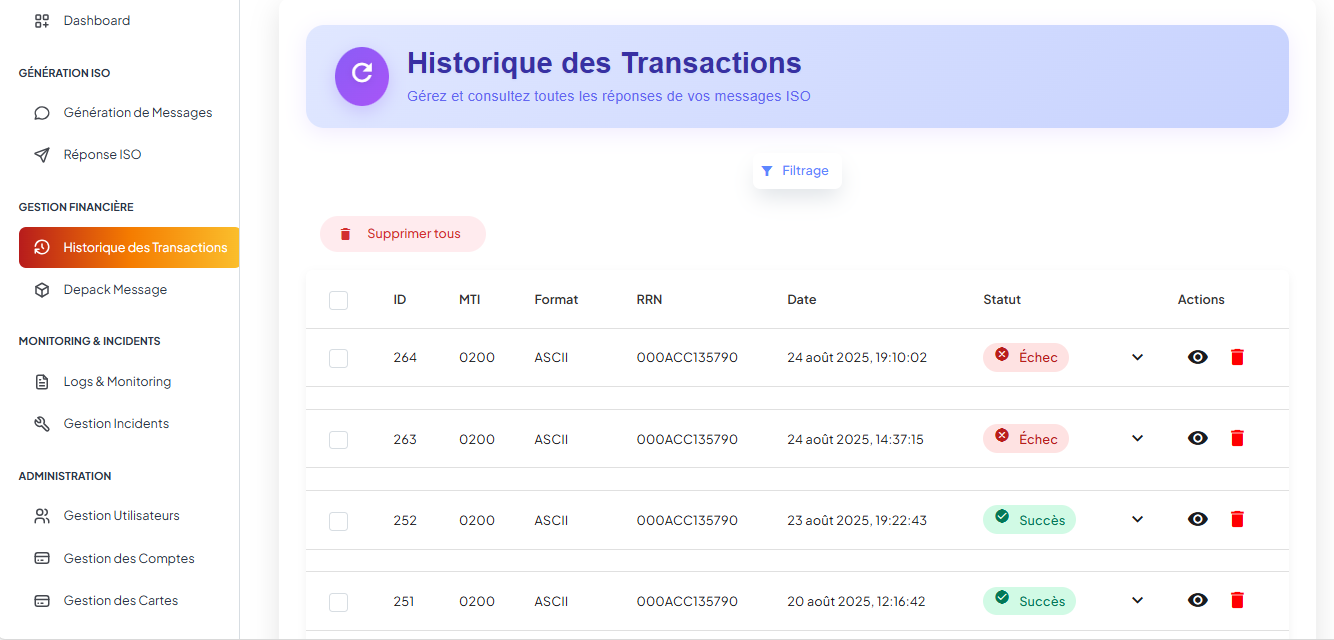
\includegraphics[width=1\textwidth]{figures/images/Historique.png}
\caption{Interface d'historique des transactions}
\label{fig:interface-historique-transactions}
\end{figure}



\paragraph{} 
Cette interface est dédiée à la consultation et à la gestion de l'historique complet des transactions ISO traitées par le système. Elle permet aux utilisateurs de visualiser toutes les réponses aux messages ISO envoyés, offrant ainsi une vue d'ensemble des opérations financières et facilitant le suivi et l'audit des transactions.

\paragraph{} 
L'interface présente un tableau détaillé listant chaque transaction avec des informations essentielles. Chaque ligne est accompagnée de cases à cocher permettant la sélection multiple de transactions.

\paragraph{} 
Trois fonctionnalités principales sont disponibles : la suppression (individuelle ou en masse) des transactions, le filtrage pour affiner la recherche selon des critères spécifiques, et le téléchargement des rapports dans différents formats (PDF, Excel, CSV) pour l'export et l'archivage des données.


\subsection{Interface d'historique des transactions}

\begin{figure}[H]
\centering
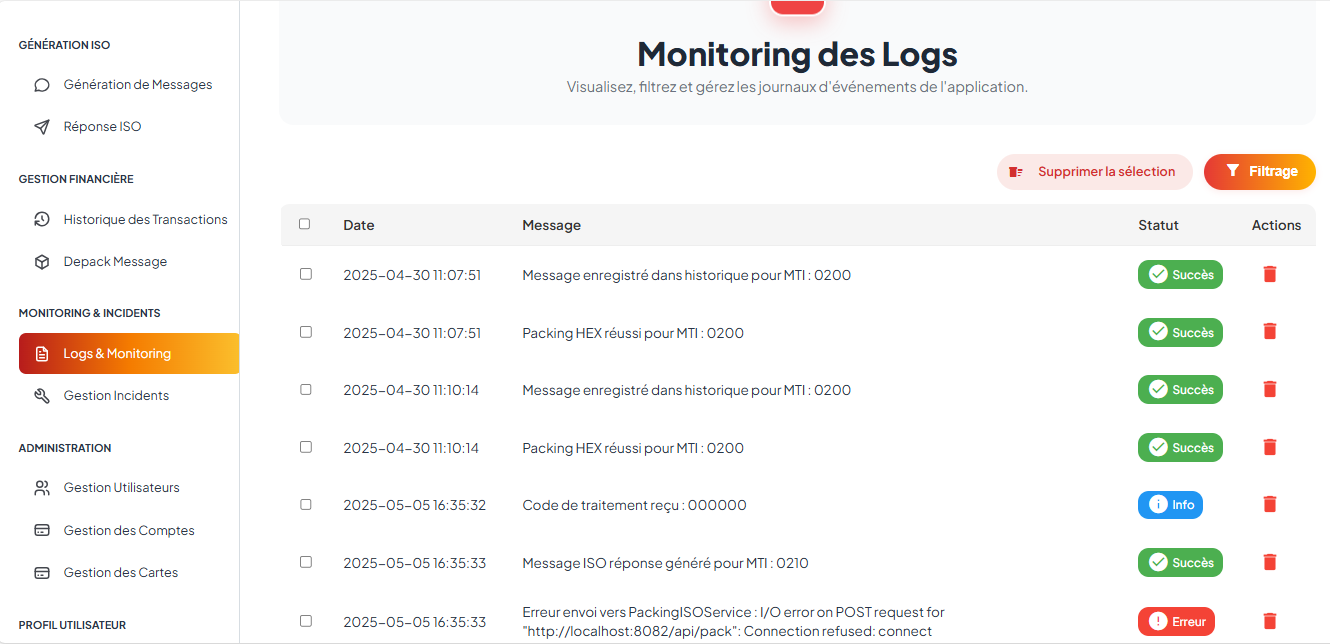
\includegraphics[width=1\textwidth]{figures/images/Logs.png}
\caption{Interface de Monitoring des Logs de l'application HPS}
\label{fig:mobile_app_architecture}
\end{figure}

Cette interface est dédiée à la visualisation, au filtrage et à la gestion des journaux d'événements de l'application HPS. Elle offre une vue centralisée des activités du système, permettant aux administrateurs et aux testeurs de consulter les logs en temps réel, d'identifier les succès, les informations importantes et les erreurs, facilitant ainsi le débogage et la maintenance.

L'interface propose des fonctionnalités de suppression (individuelle ou en masse) des logs et de filtrage selon différents critères (date, statut). Elle affiche les journaux d'événements avec la date et l'heure précises, le message détaillé et le statut de l'événement (Succès, Info, Erreur) pour une surveillance efficace du système.


    


\subsection{Interface de déclaration d'incident}


\begin{figure}[H]
\centering
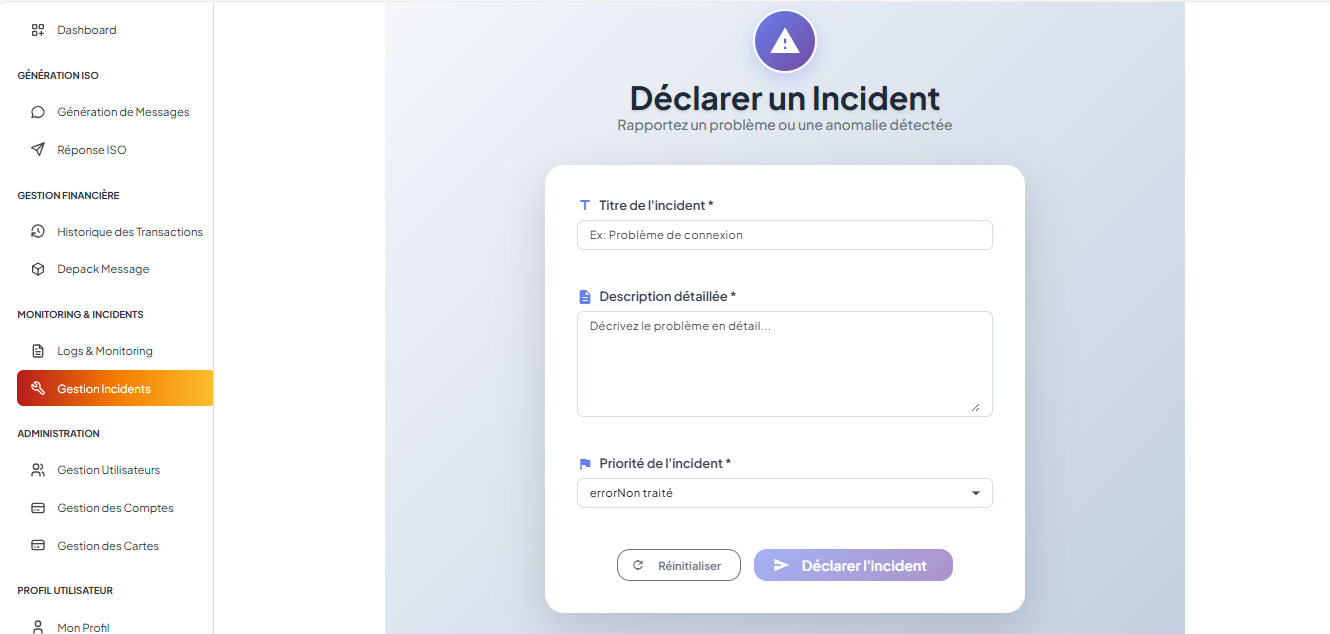
\includegraphics[width=1\textwidth]{figures/images/Incident.png}
\caption{Interface de déclaration d'incident}
\label{fig:mobile_app_architecture}
\end{figure}

Cette interface est dédiée à la déclaration et au signalement des problèmes ou anomalies détectées au sein de l'application HPS. Elle offre un formulaire structuré permettant aux utilisateurs de documenter précisément les incidents, facilitant ainsi leur suivi et leur résolution par les équipes techniques.

\begin{enumerate}[label=\alph*)]
\item \textbf{Interface de gestion des incidents} \\

\begin{figure}[H]
\centering
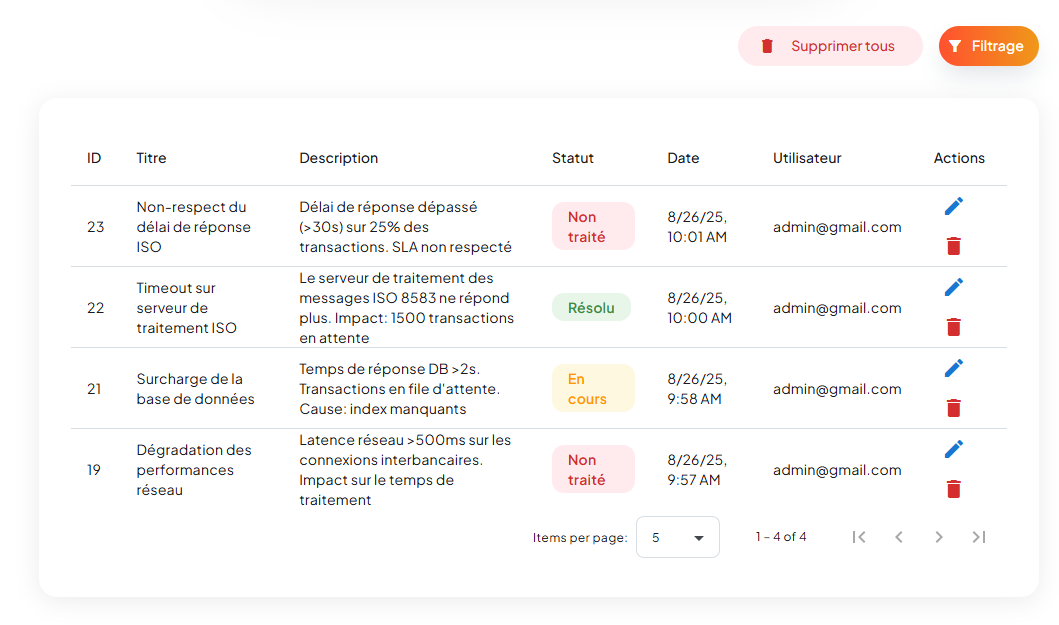
\includegraphics[width=1\textwidth]{figures/images/Tincident.png}
\caption{Interface de gestion des incidents}
\label{fig:mobile_app_architecture}
\end{figure}

Cette interface est dédiée à la consultation, au suivi et à la gestion des incidents déclarés au sein de l'application HPS. Elle offre une vue centralisée et organisée des problèmes détectés, permettant aux administrateurs et aux équipes de support de surveiller leur statut, d'identifier les causes et de prendre les mesures correctives nécessaires.


\item \textbf{Système de notification par email des incidents} \\

\begin{figure}[H]
\centering
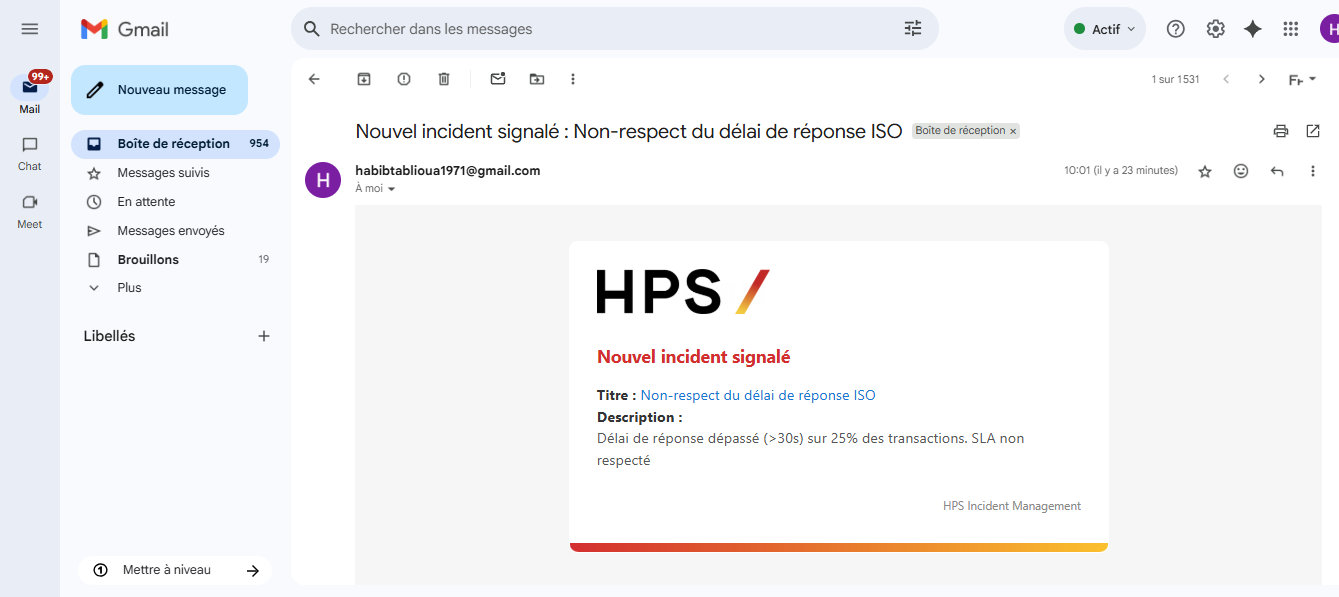
\includegraphics[width=1\textwidth]{figures/images/Email.png}
\caption{Interface de notification par email d'un incident déclaré}
\label{fig:mobile_app_architectur}
\end{figure}

la figure (\ref{fig:mobile_app_architectur}) illustre le système de notification automatique par email qui s'active lorsqu'un testeur enregistre un incident dans l'application HPS. Dès qu'un incident est déclaré, le système génère et envoie automatiquement un email de notification à l'administrateur pour l'informer de la détection d'un nouveau problème.

\end{enumerate}


\subsection{Interface de gestion des utilisateurs}


\begin{figure}[H]
\centering
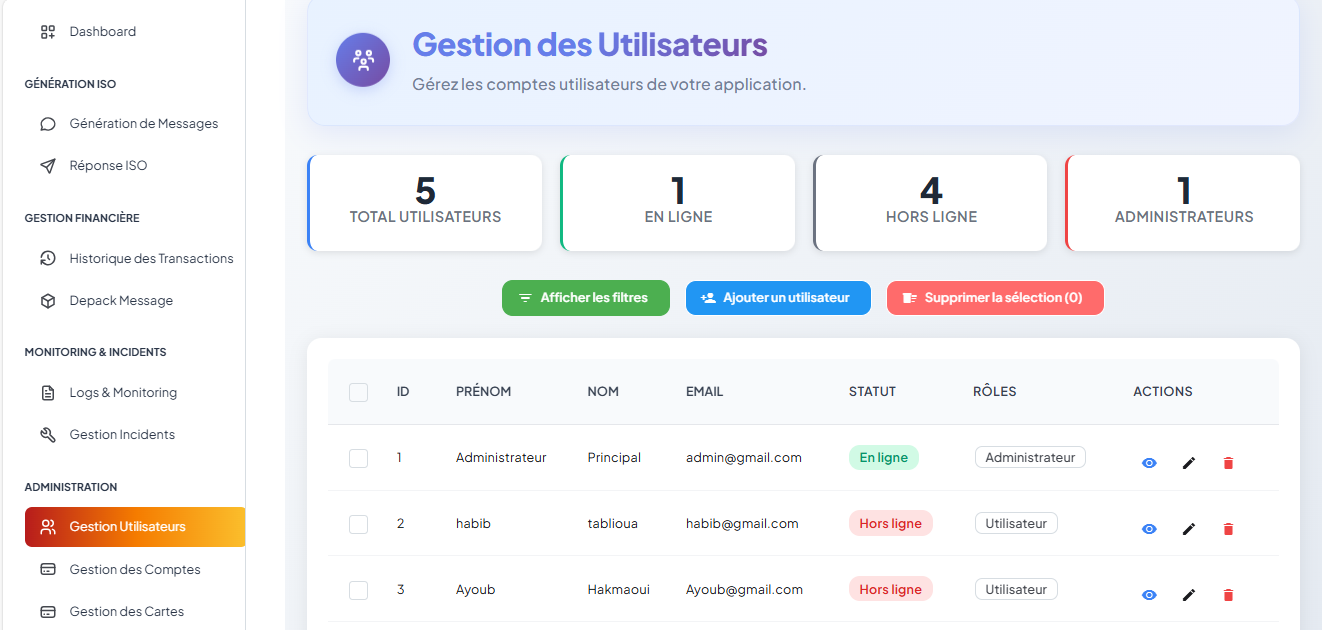
\includegraphics[width=1\textwidth]{figures/images/GestionUtilisateure.png}
\caption{Interface de gestion des utilisateurs}
\label{fig:mobile_app_architecture}
\end{figure}

Cette interface est dédiée à la gestion complète des comptes utilisateurs de l'application HPS. Elle offre aux administrateurs une vue centralisée et organisée de tous les utilisateurs du système, permettant de surveiller leur statut, gérer leurs rôles et effectuer des opérations d'administration sur leurs comptes.

\subsection{Interface de gestion des comptes bancaires}


\begin{figure}[H]
\centering
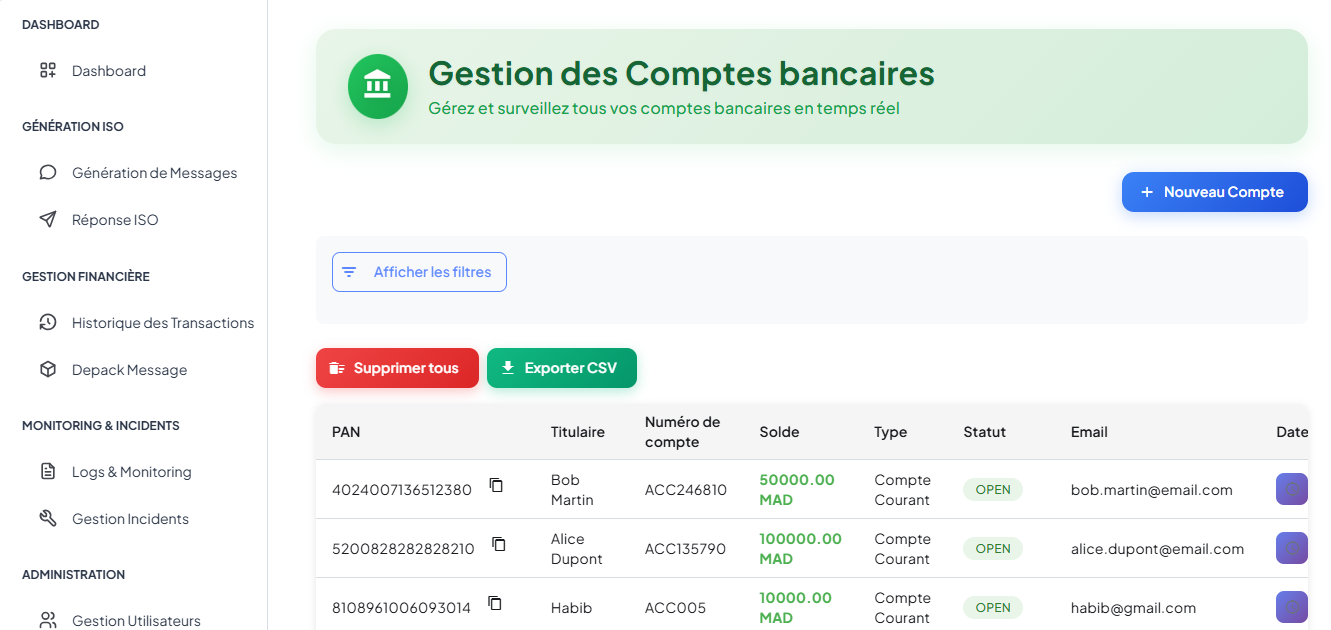
\includegraphics[width=1\textwidth]{figures/images/CompteB.png}
\caption{Interface de gestion des comptes bancaires}
\label{fig:mobile_app_architecture}
\end{figure}

Cette interface est dédiée à la gestion et au suivi en temps réel de toutes les cartes bancaires. Elle offre une vue centralisée et complète, permettant aux administrateurs de consulter les détails des cartes, de surveiller leur statut et d'effectuer des opérations administratives essentielles.


\subsection{Interface de gestion des cartes bancaires}


\begin{figure}[H]
\centering
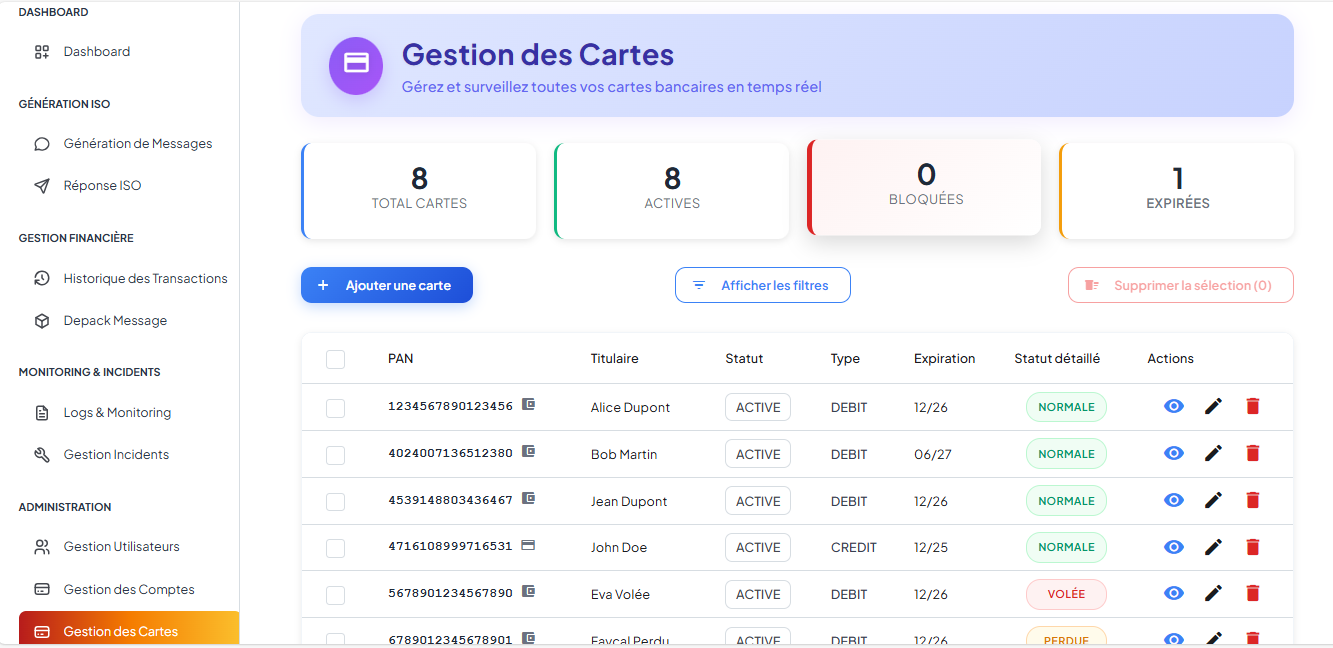
\includegraphics[width=1\textwidth]{figures/images/Carte.png}
\caption{Interface de gestion des cartes bancaires}
\label{fig:mobile_app_architecture}
\end{figure}

Cette interface est dédiée à la gestion et au suivi en temps réel de toutes les cartes bancaires. Elle offre une vue centralisée de toutes les cartes, permettant aux administrateurs de consulter les détails et de gérer les informations des cartes bancaires.


\subsection{ Interface de profil utilisateur}


\begin{figure}[H]
\centering
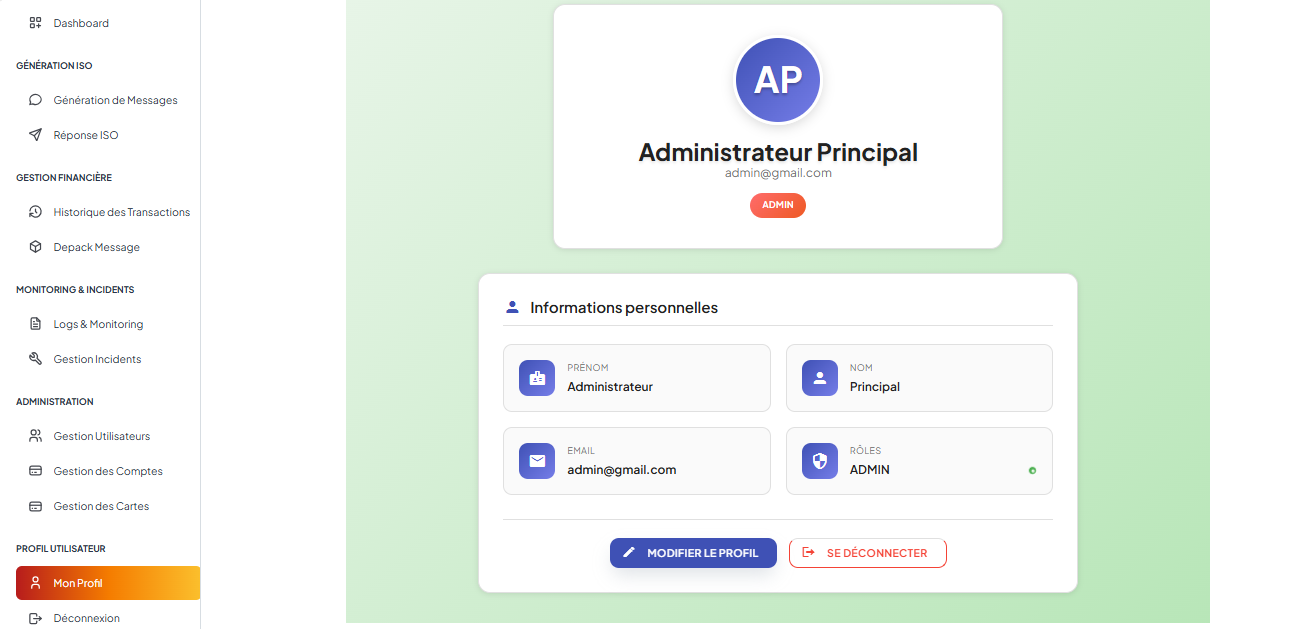
\includegraphics[width=1\textwidth]{figures/images/Profile.png}
\caption{Interface de profil utilisateur}
\label{fig:mobile_app_architecture}
\end{figure}

Cette interface est dédiée à la consultation et à la gestion du profil de l'utilisateur connecté. Elle offre une vue centralisée des informations personnelles et des rôles attribués, permettant à chaque utilisateur (administrateur ou testeur) de visualiser ses détails et d'accéder aux options de modification ou de déconnexion.


\section*{Conclusion}
Ce volet m'a permis de mettre en lumière la mise en œuvre pratique de mon projet. Grâce à une présentation détaillée des interfaces utilisateur, j'ai posé les bases solides nécessaires à la réalisation effective de mon application. Cette étape de réalisation a été fondamentale pour concrétiser les spécifications techniques définies précédemment et démontrer la faisabilité de la solution proposée. La mise en place de ces interfaces a également permis de valider l'architecture technique choisie et d'identifier les améliorations potentielles pour optimiser l'expérience utilisateur et la performance du système.






